\documentclass[12pt,twoside]{article}   
\usepackage{light}

%\hidesolutions
\showsolutions

\newcommand{\hint}[1]{({\it Hint: #1})}
\newcommand{\card}[1]{\left|#1\right|}

\begin{document}
\problemset{0}{October 4, 2010}{Sample midterm problem}

%%%%%%%%%%%%%%%%%%%%%%%%%%%%%%%%%%%%%%%%%%%%%%%%%%%%%%%%%%%%%%%%%%%%%%%%%%%%%%%


%number theory

\begin{problem}{20}
Define a number
$S_p = 1^p + 2^p +3^p + \ldots (p-1)^p.$
You will show in this problem that if $p$ is an odd prime, then $p|S_p$.
\bparts
\ppart{10}
 Use Fermat's Theorem to show that $S_p \equiv 1+2+\ldots + (p-1) \pmod p$.
\solution
{
\begin{eqnarray*}
S_p &\equiv& 1^p + 2^p + \ldots (p-1)^p\\
& \equiv& 1\cdot1^{p-1} + 2\cdot2^{p-1} + \ldots + (p-1)\cdot (p-1)^{p-1}\\
& \equiv& 1\cdot 1 + 2 \cdot 1 + \ldots + (p-1) \cdot 1\\
& \equiv & 1 + 2 + \ldots + (p-1) \pmod p
\end{eqnarray*}
}
\ppart{10}
Show that $p|(1+2+\ldots + (p-1))$ and explain why this implies that $p$ divides $S_p$.
\solution{
$1+2+\ldots + (p-1) = \frac{(p-1)p}2.$\\
$p$ is odd, so $p-1$ is even, which means $\frac{p-1}2$ is some integer $k$. Therefore
\[1+2+\ldots + (p-1) = kp,\]
so $p|(1+2+\ldots + (p-1))$. As a consequence, $1+2+\ldots + (p-1) \equiv 0 \pmod p$. Therefore
\[S_p \equiv 1+2+\ldots + (p-1) \equiv 0 \pmod p,\]
so $p|S_p$.
}
\eparts
\end{problem}

\begin{problem}{20}
Suppose $S(n)$ is a predicate on natural numbers, $n$, and suppose
\begin{equation}\label{Sk2}
\forall k \in \mathbb{N} \; S(k) \implies S(k+2).
\end{equation}
If~(\ref{Sk2}) holds, some of the assertions below must \emph{always}
(\textbf{A}) hold, some \emph{can} (\textbf{C}) hold but not always,
and some can \emph{never} (\textbf{N}) hold.  Indicate which case
applies for each of the assertions by \textbf{circling} the correct
letter.

\bparts

\ppart{2}  \hspace{.2in} {\bf A C N \hspace{.2in}} 
$\forall n \ge 0\; S(n)$ 
\solution{\textbf{C}.
The assertion means that $S$ is always true.  So $S(k+2)$ is always true, and
therefore $S(k) \implies S(k+2)$ is always true.  So this case is possible.
But~\ref{Sk2} also holds when $S$ is always false, so the asertion does not
always hold when \ref{Sk2} does}

\ppart{2} \hspace{.2in} {\bf A C N \hspace{.2in}} $\neg{S(0)}
\land \forall n \ge 1\; S(n)$ 
\solution{\textbf{C}.
This time $S$ is false at 0, but true everywhere else.  So $S(k) \implies
S(k+2)$ still always holds because $S(k+2)$ is still always true.  So this
assertion can hold, but not always, since~(\ref{Sk2}) can hold when $S(0)$ is
true.}

\ppart{2}  \hspace{.2in} {\bf A C N \hspace{.2in}} 
$\forall n \ge 0\; \neg{S(n)}$
\solution{\textbf{C.}
Now $S$ is always false.  So $S(k) \implies S(k+2)$ is always true because
$S(k)$ is false.  So this case is possible, but again does not always hold.}

\ppart{2}  \hspace{.2in} {\bf A C N \hspace{.2in}} 
$(\forall n \le 100\; S(n)) \land (\forall n > 100\; \neg{S(n)})$ 
\solution{\textbf{N}.
In this case, $S$ is true for $n$ up to 100 and false from 101 on.  So $S(99)$
is true, but $S(101)$ is false.  That means that $S(k) \not \implies S(k+2)$
for $k = 99$.  This case is impossible.}

\ppart{2} \hspace{.2in} {\bf A C N \hspace{.2in}} $(\forall n
\le 100\; \neg{S(n)}) \land (\forall n > 100\; S(n))$ 
\solution{\textbf{C}.
In this case, $S$ is false for $n$ up to 100 and true from 101 on.  So $S(k)
\implies S(k+2)$ for $k \le 100$ because $S(k)$ is false, and $S(k) \implies
S(k+2)$ for $k \ge 99$ because $S(k+2)$ is true.  So this case is possible, but
again does not always hold}

\ppart{2}  \hspace{.2in} {\bf A C N \hspace{.2in}} 
$S(0) \implies \forall n\ S(n+2)$ 
\solution{\textbf{C}.
If $S(n)$ is always true this assertion holds.  So this case is possible.  If
$S(n)$ is true only for even $n$~(\ref{Sk2}) still holds, but $S(1+2)$ is
false.  So this case does not always hold.}

\ppart{2}  \hspace{.2in} {\bf A C N \hspace{.2in}} 
$S(1) \implies \forall n\ S(2n+1)$
\solution{\textbf{A}.
This assertion says that if $S(1)$ holds, then $S(n)$ holds for all odd $n$.
This case is always true.}

\ppart{2}  \hspace{.2in} {\bf A C N \hspace{.2in}} 
$[\exists n\, S(2n)] \implies \forall n \ S(2n+2)$
\solution{\textbf{C}.
If $S(n)$ is always true, this assertion holds.  So this case is possible.  If
$S(n)$ is true only for even $n$ greater than 4,~(\ref{Sk2}) holds, but this
assertion is false. So this case does not always hold.}

\ppart{2}  \hspace{.2in} {\bf A C N \hspace{.2in}} 
$\exists n\, \exists m > n\, [S(2n) \land \neg{S(2m)}]$
\solution{\textbf{N}.
This assertion says that $S(n)$ holds for some even number ($2n$) but not for
some other larger even number ($2m$).  However, if $S(2n)$ holds, we can
apply~(\ref{Sk2}) $n-m$ times to conclude $S(2m)$ also holds.  This case is
impossible.}

\ppart{2}  \hspace{.2in} {\bf A C N \hspace{.2in}} 
$[\exists n\, S(n)] \implies \forall n\, \exists m> n\, S(m)$
\solution{\textbf{A}.
This assertion says that if $S(n)$ holds for some $n$, then for every number,
there is a larger number $m$ for which $S(m)$ also holds.  Since~(\ref{Sk2})
implies that if there is one $n$ for which $S(n)$ holds, there are an infinite,
increasing chain of $k$s for which $S(k)$ holds, this case is always true.}

\iffalse
\ppart{2}  \hspace{.2in} {\bf A C N \hspace{.2in}} 
$\neg{S(0)} \implies \forall n \ \neg{S(2n)}$
\fi

\eparts
\end{problem}

\begin{problem}{20}
% Strong Induction

Let $G_0=1$, $G_1=2$, $G_2=4$, and define
\begin{equation}\label{Pn}
G_n =  G_{n-1} +2G_{n-2} + G_{n-3}
\end{equation}
for $n \geq 3$.  Show by induction that $G_n\leq \paren{2.2}^n$ for all $n \geq
0$.

\solution{

The proof is by strong induction with hypothesis $P(n) := G_n\leq \paren{2.2}^n$.

\begin{proof}
\textbf{Base Cases}

\textbf{$n=0$:} $G_0 = 1 = \paren{2.2}^0$.

\textbf{$n=1$:} $G_1 = 2 < 2.2 = \paren{2.2}^1$.

\textbf{$n=2$:} $G_2 =f 4 < 4.84 = \paren{2.2}^2$.

\textbf{Inductive Step}:
Assume $n \geq 2$ and $P(k)$ for all $k$ such that $0 \leq k \leq n$.
\begin{align*}
G_{n+1}
& = G_n +2G_{n-1} + G_{n-2} & \text{by~\eqref{Pn}}\\
& \leq (2.2)^n + 2(2.2)^{n-1} + (2.2)^{n-2} & \text{by induction hypothesis}\\
& = (2.2)^{n-2} [(2.2)^2 + 2(2.2) + 1]\\
& = (2.2)^{n-2} [(2.2 + 1)^2]\\
& = (2.2)^{n-2} (3.2)^2\\
& = (2.2)^{n-2} (10.24)\\
& < (2.2)^{n-2} (10.648)\\
& = (2.2)^{n-2} (2.2)^3\\
& = (2.2)^{n+1}
\end{align*}
\end{proof}
}
\end{problem}

%based on Fall 02, but changed
\begin{problem}{20}
The $6.042$ professors are planning to have a midterm exam and want the midterm grades to be recognized by the EECS department. This requires the completion of a number
tasks, each of which takes one hour to complete.  The prerequisites associated with these tasks are
listed below.
\begin{center}
\begin{tabular}{cll}
\textsc{Abbrv.} & \textsc{Task} & \textsc{Prerequisites} \\
S & Hold an ice cream study session & I,A\\
W & Write midterm questions &  I (for the TAs)\\
M & Schedule a make-up exam & A \\
G & Grade the midterms & H,U\\
A & Announce the midterm date &  \\
H & Hold the midterm & W,R,S \\
I & Buy ice cream &  \\
R & Release a sample midterm &  \\
U & Hold the make-up exam & H,M 
\end{tabular}
\end{center}

\bparts

\ppart{4} Draw the Hasse diagram for the tasks and their
prerequisites.
  
\solution{
\begin{center}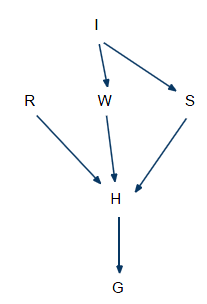
\includegraphics{hasse_diagram.png}\end{center}
}

\ppart{2} Give one ordering of the tasks that will fulfill the department's prerequisites.
\solution{
I A R W S M H U G
}

\ppart{2} The professors have decided that since their TAs are quite
smart and they have so many of them, they can get as many tasks done at a time as
they wish.  What is the minimum amount of time required for them to
finish all the tasks?

\solution{The minimum required time is 5 (length of the critical path
 I-W-H-U-G)}

\eparts

It turns out that the graph is actually far more complicated than the
one above.  In fact, the professors don't know what the actual diagram is because the department forgot to tell them.  All the professors have been told is that they must
complete $n$ tasks, each of which takes 1 hour, and that they are allowed to hire at most $t$ TAs, since they will never be able to use more of them at a given time anyway.  Without knowing
anything more about the actual graph, the professors are trying to figure out how
much time they will need to complete all the tasks.  A TA can only complete one task in 1
hour, but has the stamina to work for days on end.  Let $n$ and $t$ be
fixed, and $n>t>1$.

\bparts
\ppart{6} Write a simple formula in $n$ and $t$ for the minimum number of time the professors have to allow for all the tasks in order to be \emph{guaranteed}
to finish assuming that they have $t$ TAs.

\solution{There are $n$ tasks, $t$ is the longest antichain.  We are
guaranteed that everything can be partitioned into $t$ chains.

$n-t+1$.  In the worst case there could be a chain of size
$n-t+1$ but no larger, which means that if the professors start $n-t+1$ hours before whatever deadline they have, they'll be set.
}

\ppart{6} Write a simple formula in $n$ and $t$ for the smallest
number of time they could give themselves and still \emph{possibly} finish on of time.  (That is, if they give themselves less time, they will
never be able to finish on time using $t$ TAs, no matter
how ``favorable'' the graph turns out to be.)

\solution{$\ceil{n/t}$.  Since there is no antichain of size $t+1$, we know
that at least one chain must have $\geq n/t$ elements.  If the professors
give themselves less than $\ceil{n/t}$ hours, this chain will not be completed on time.}
\eparts
\end{problem}

\end{document}
